\documentclass{beamer}
\usetheme{metropolis}           % Use metropolis theme

\usepackage{tikz}
\usetikzlibrary{positioning}
\usepackage{lscape}
\usepackage{bm}
\usepackage{ulem}
\usepackage{amssymb}

\title{Understanding the Stochastic Partial Differential Equation Approach to Smoothing}
\date{17 June 2021}
\author{\textbf{David L. Miller} \and Richard Glennie \and Andrew Seaton}
\institute{International Biometric Society Journal Club}
\begin{document}
\maketitle

\begin{frame}{Andy and Richard}
  \begin{figure}[h]
    \begin{center}
          
\includegraphics[width=0.45
          \textwidth]{figures/andy.jpg} 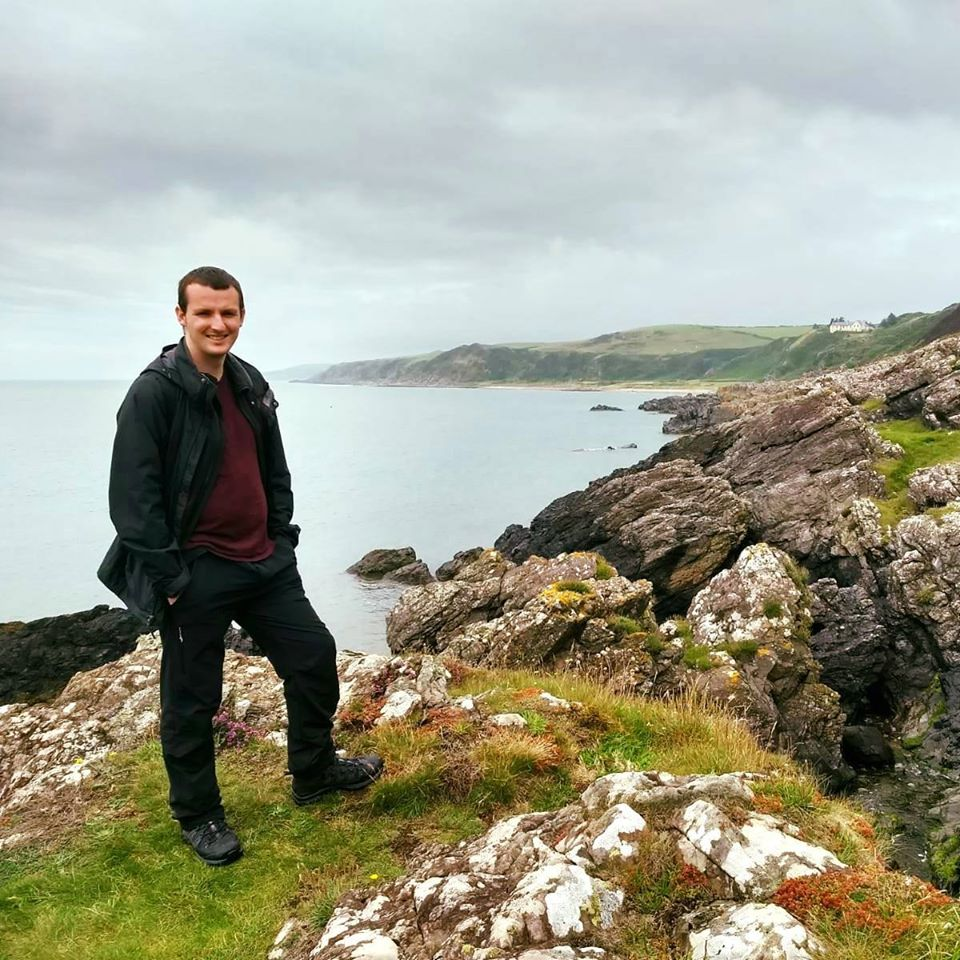
\includegraphics[width=0.45\textwidth]{figures/richard.jpg}
    \end{center}
  \end{figure}
\end{frame}

% 2 column template, if needed
%  \begin{columns}
%    \begin{column}{0.48\textwidth}
%       boop
%    \end{column}
%    \begin{column}{0.48\textwidth}
%       boop
%    \end{column}
%  \end{columns}

% should be some rough intro material here
\section{Introduction}

\begin{frame}{The kinds of data we'll talk about}
  \begin{figure}[h]
    \begin{center}
      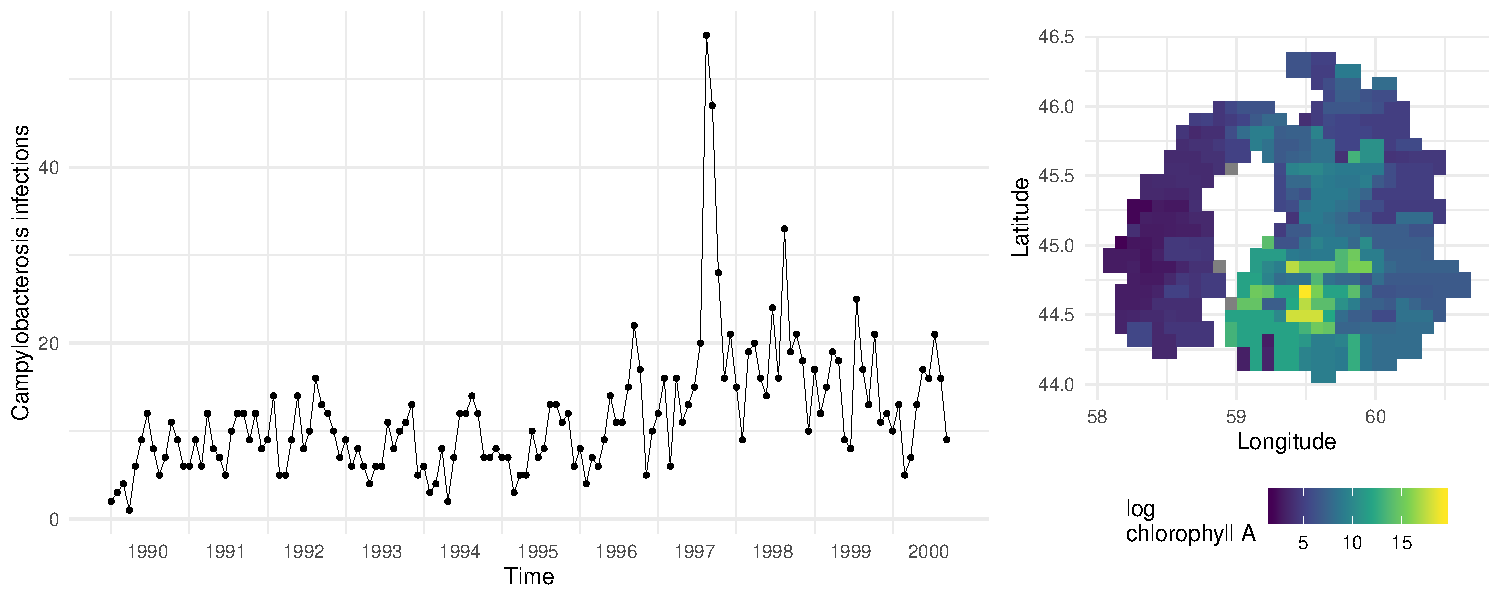
\includegraphics[width=\textwidth]{figures/ex_data.pdf}
    \end{center}
  \end{figure}
\end{frame}


\begin{frame}{How to model dependence?} 

\textbf{Tobler's law}: ``everything is related to everything else, but near things are more related than distant things."

Two ways to think about this: \textit{Smoothness} and \textit{Correlation}. 

  \begin{figure}[h]
    \begin{center}
      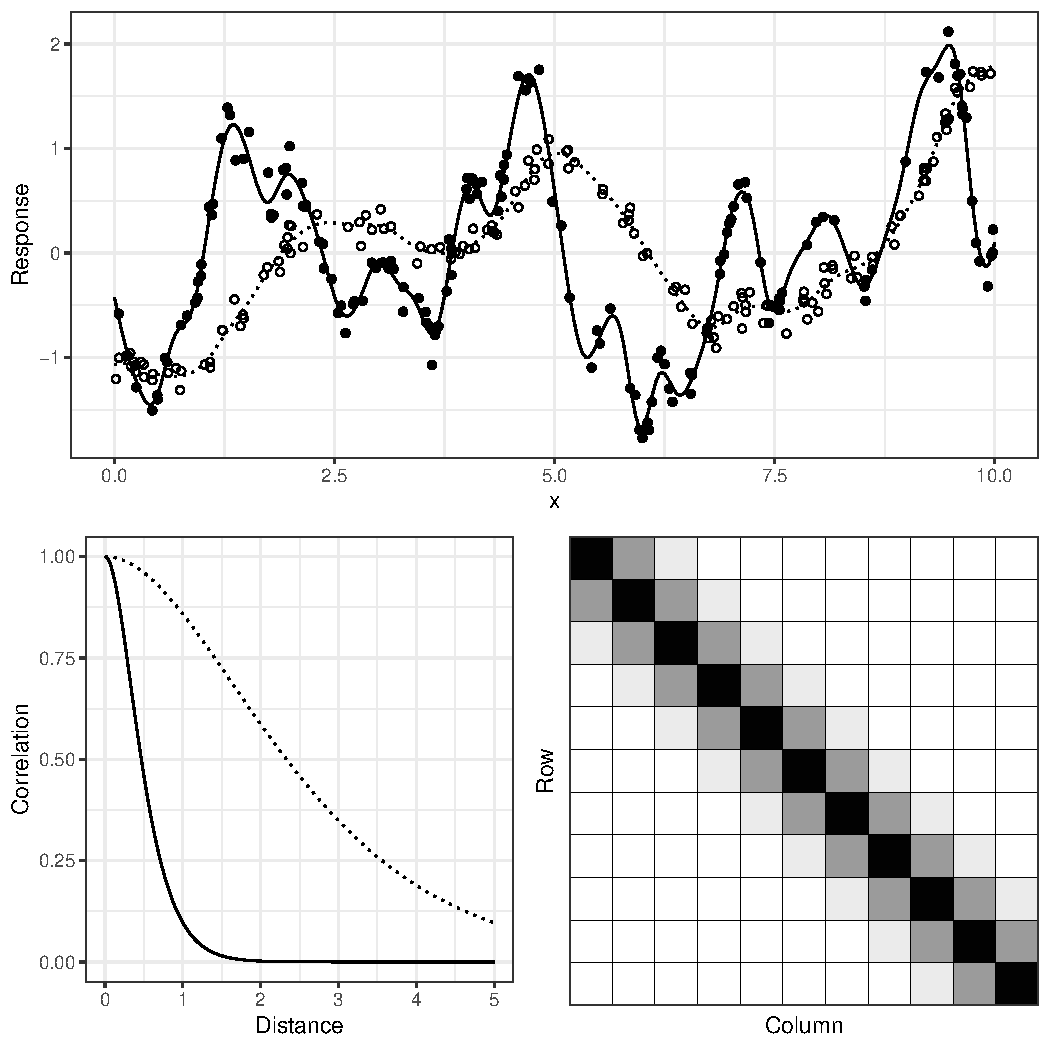
\includegraphics[width=0.7\textwidth, trim={0 9cm 0 0}, clip]{figures/smooth_corr.pdf}
    \end{center}
  \end{figure}

\end{frame}

\begin{frame}{How to model dependence?} 

Two ways to think about this: Smoothness and Correlation. 

Two popular approaches to modelling it: GAMs and SPDEs. 

\begin{itemize}
\item GAMs $\approx$ ``smoothing using spline-type things''
\item SPDEs $\approx$ ``Mat\'ern covariance approximation using SPDEs/MRFs'' 
\end{itemize}

  \begin{figure}[h]
    \begin{center}
      
\includegraphics[height=0.3\textheight]{figures/mgcv-inside.png}
            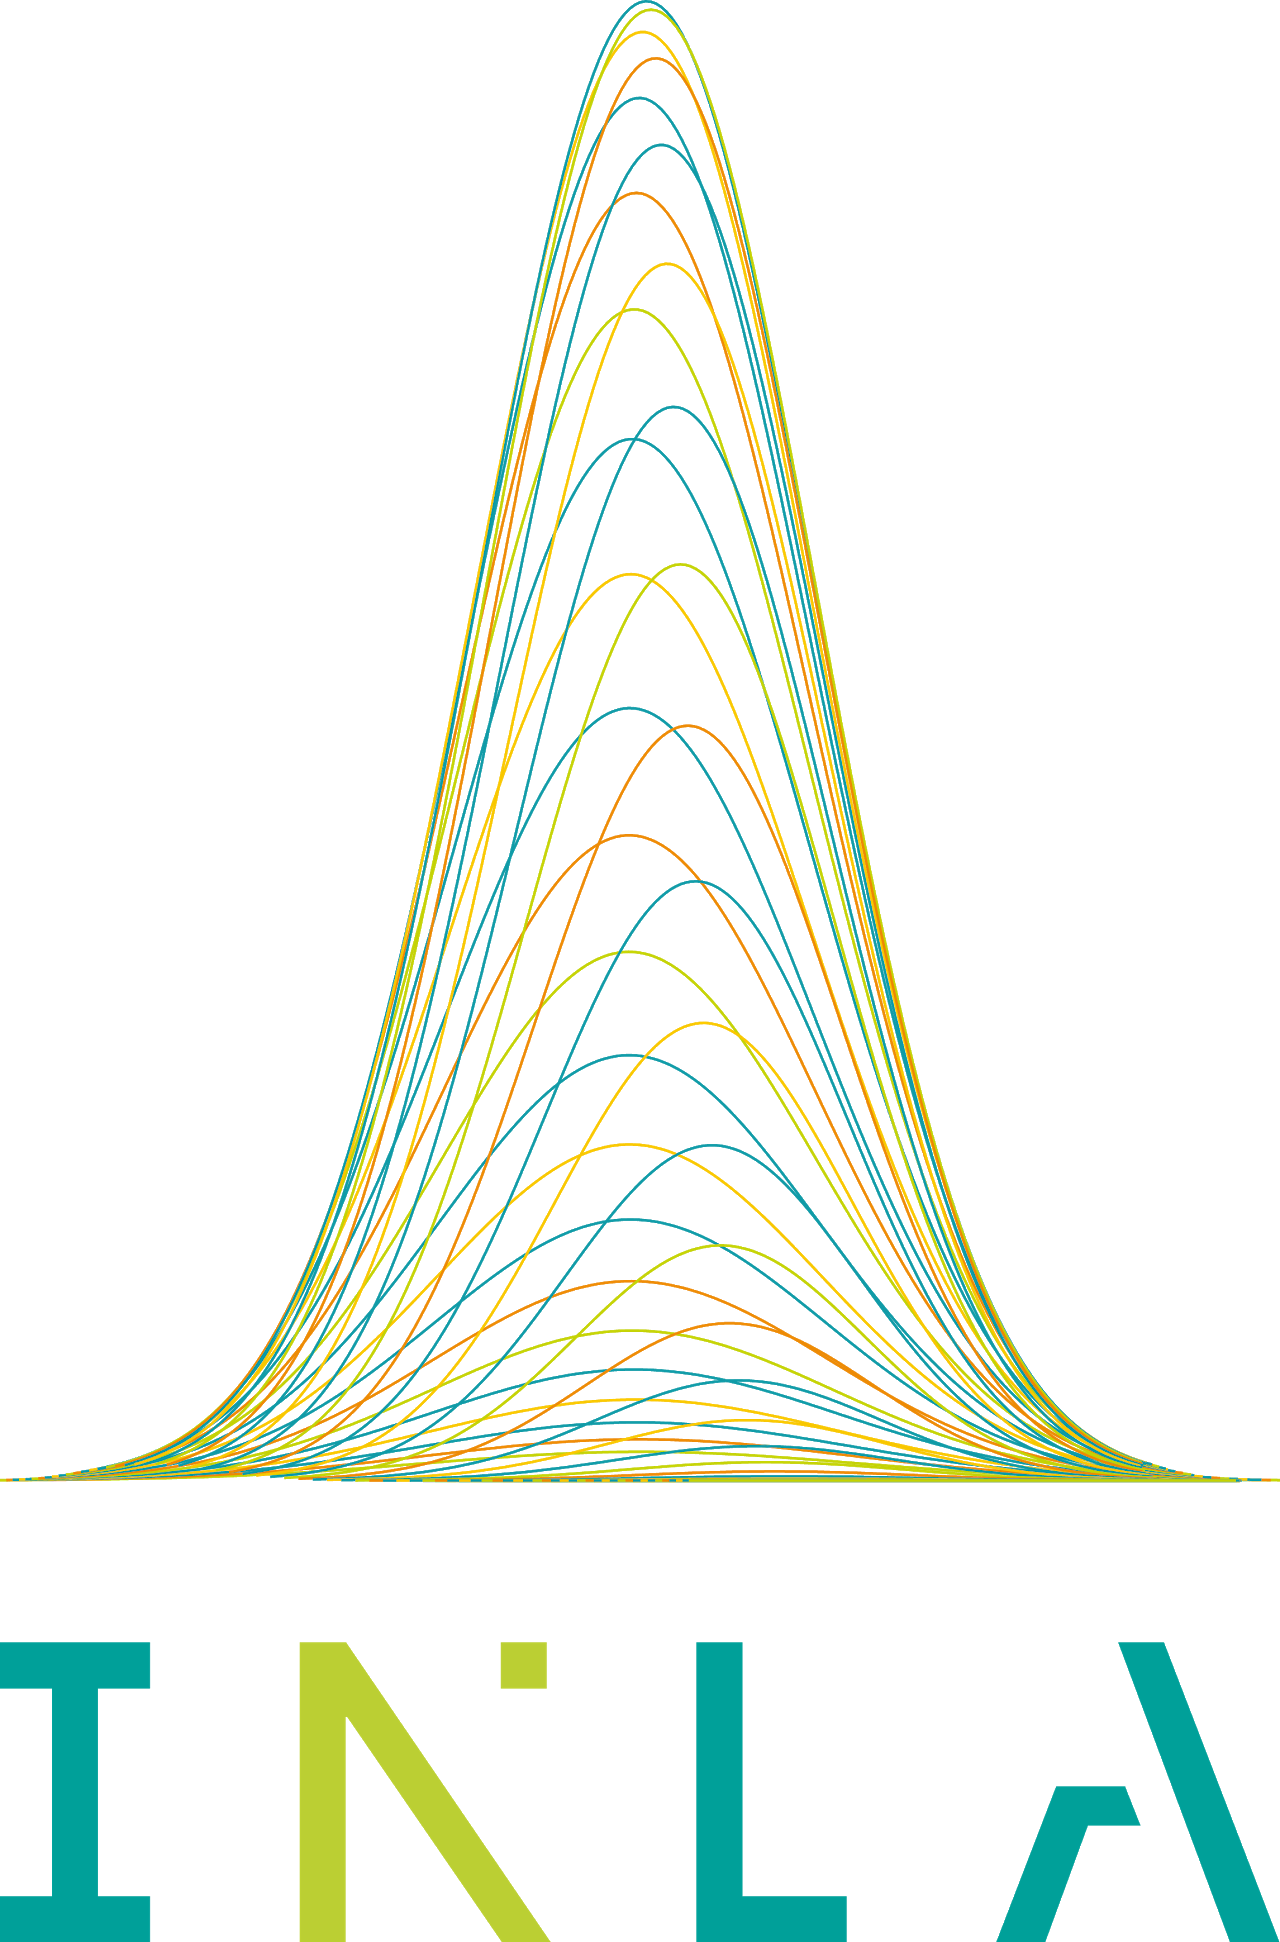
\includegraphics[height=0.3\textheight]{figures/inla.png}
    \end{center}
  \end{figure}

\end{frame}

\begin{frame}{Outline}

  \begin{figure}[t]
    \begin{center}
      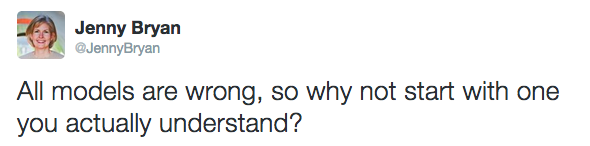
\includegraphics[width=\textwidth]{figures/jenny_models.png}
    \end{center}
  \end{figure}

{\Large
Refresh: what are GAMs made of? \\
Explain: how does the SPDE method work?\\
Apply: how can we use these results in practice?
}

\end{frame}

% explain GAMs
\section{The GAM approach}

\begin{frame}{From GLMs to GAMs}
  \begin{itemize}
    \item Want flexible, structured models
    \item GAM provides this via ``smooths''
    \item $y \sim s(x)$, where $s$ is a smooth function of $x$
  \end{itemize}
  \begin{figure}[h]
    \begin{center}
      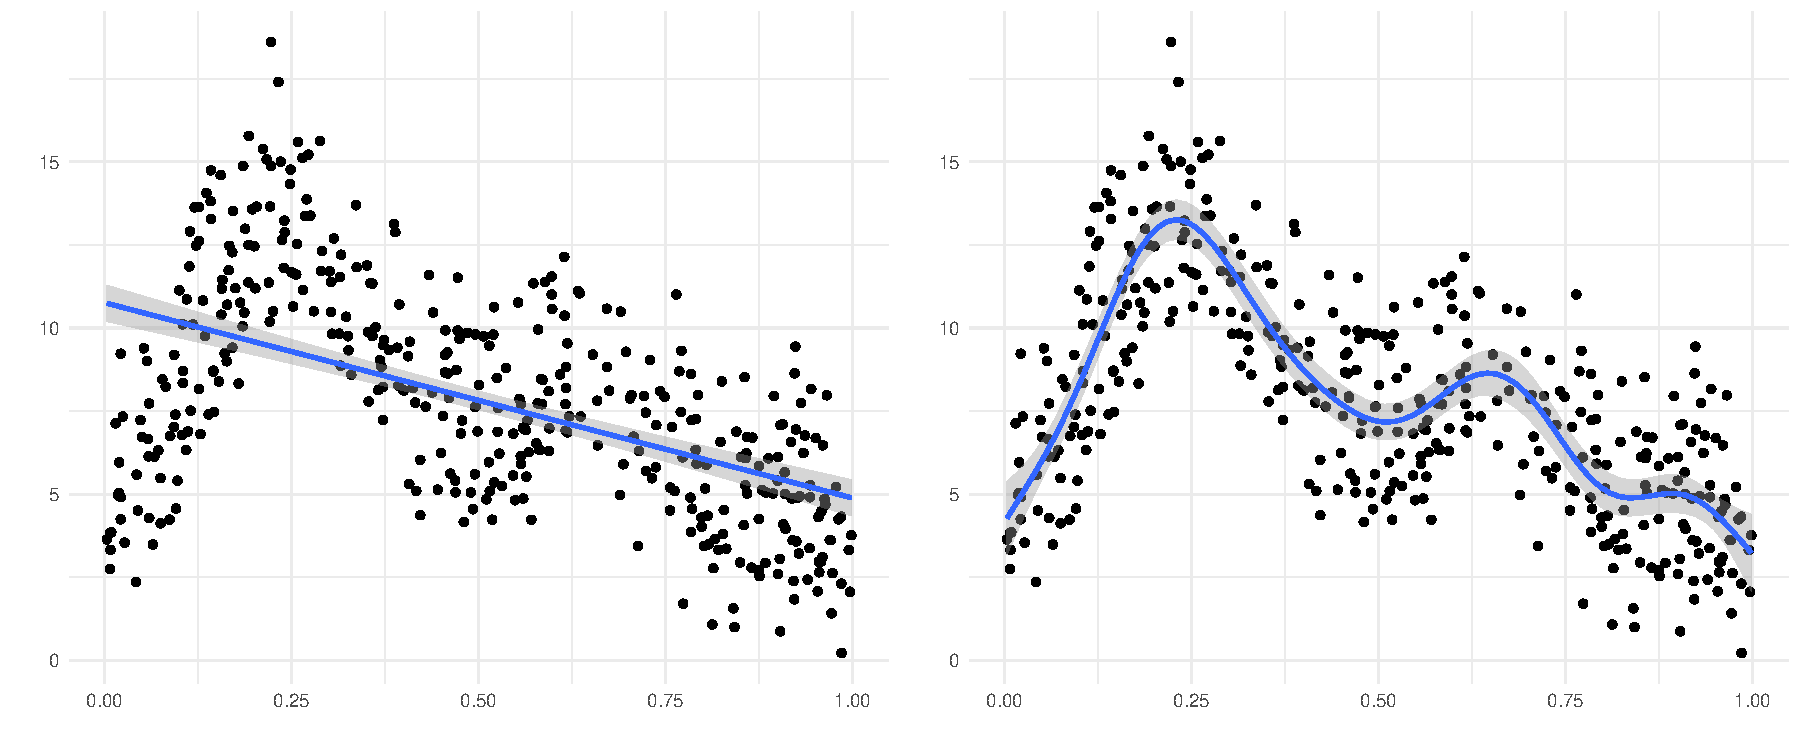
\includegraphics[width=\textwidth]{figures/lmorsmooth.pdf}
    \end{center}
  \end{figure}
\end{frame}


\begin{frame}{Examples of smooths}
  \begin{figure}[h]
    \begin{center}
      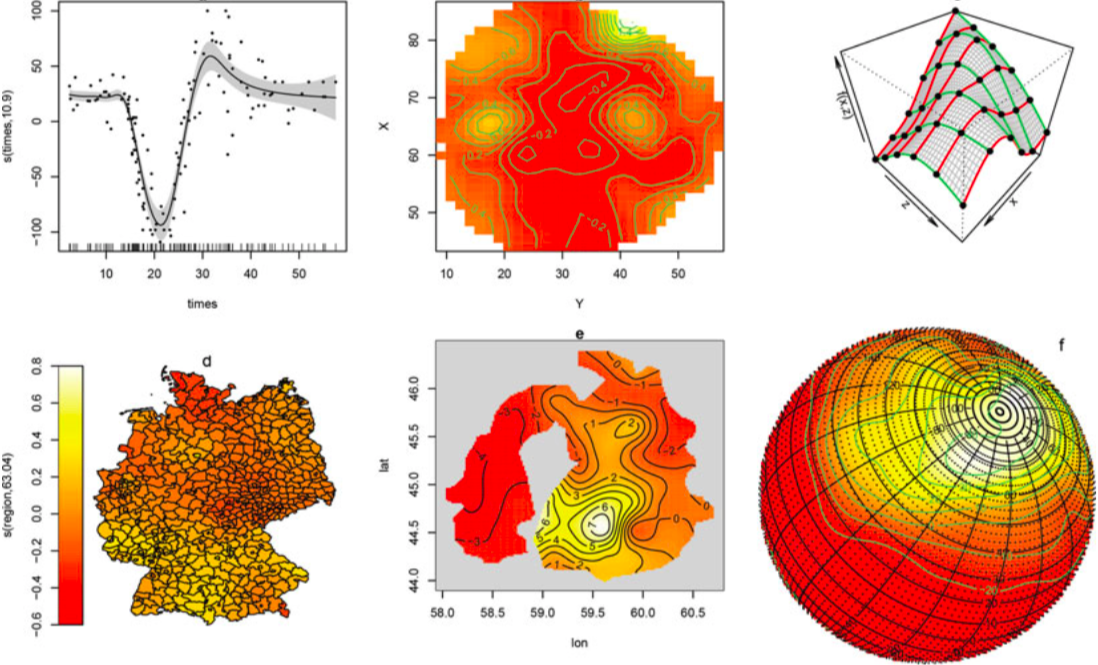
\includegraphics[width=\textwidth]{figures/smooths.png}
    \end{center}
  \end{figure}
\end{frame}

\begin{frame}{Smooths come in 2 bits\ldots}
  \begin{columns}[T]
    \begin{column}{0.40\textwidth}
      \textbf{basis functions}
      \begin{itemize}
        \item join together to make up the overall curve, $s(x)$
        \item go in the design matrix, $\textbf{X}$
      \end{itemize}
    \end{column}
    \begin{column}{0.58\textwidth}
      \textbf{penalties}
      \begin{itemize}
        \item controls how the line behaves
        \item penalty matrix $\textbf{S}$ (structure)
        \item smoothing parameter $\lambda$ (how wiggly)
      \end{itemize}
    \end{column}
  \end{columns}
  \center{\Large{``basis-penalty smoothers''}}
\end{frame}

\begin{frame}{Basis functions}
  \begin{figure}[h]
    \begin{center}
      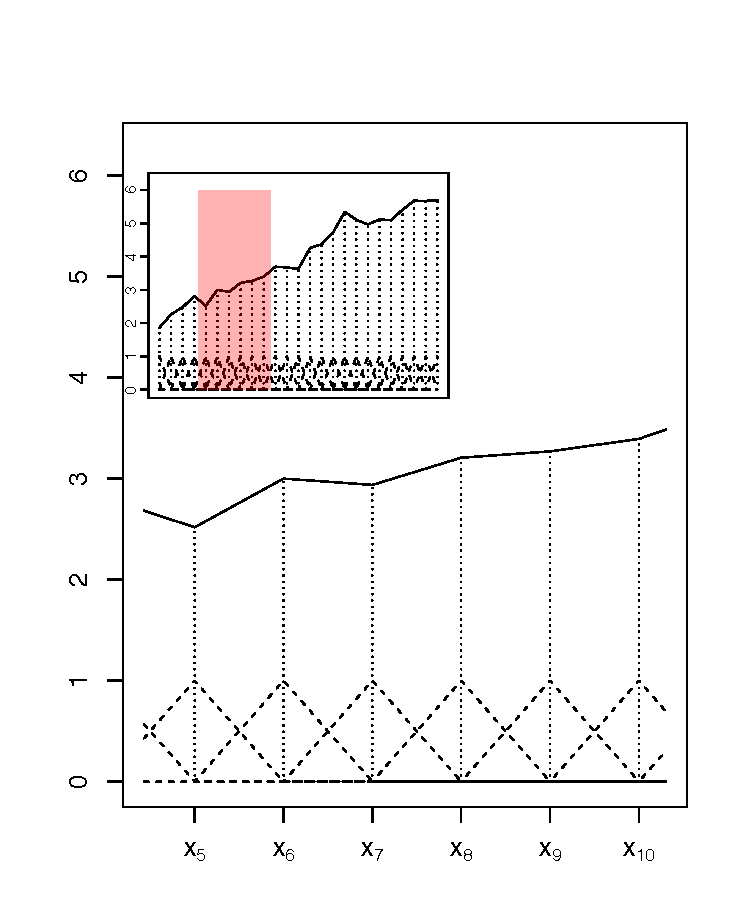
\includegraphics[height=0.9\textheight]{figures/fem.pdf}
    \end{center}
  \end{figure}
\end{frame}

\begin{frame}{Penalty and smoothing parameter}
  \begin{figure}[h]
    \begin{center}
      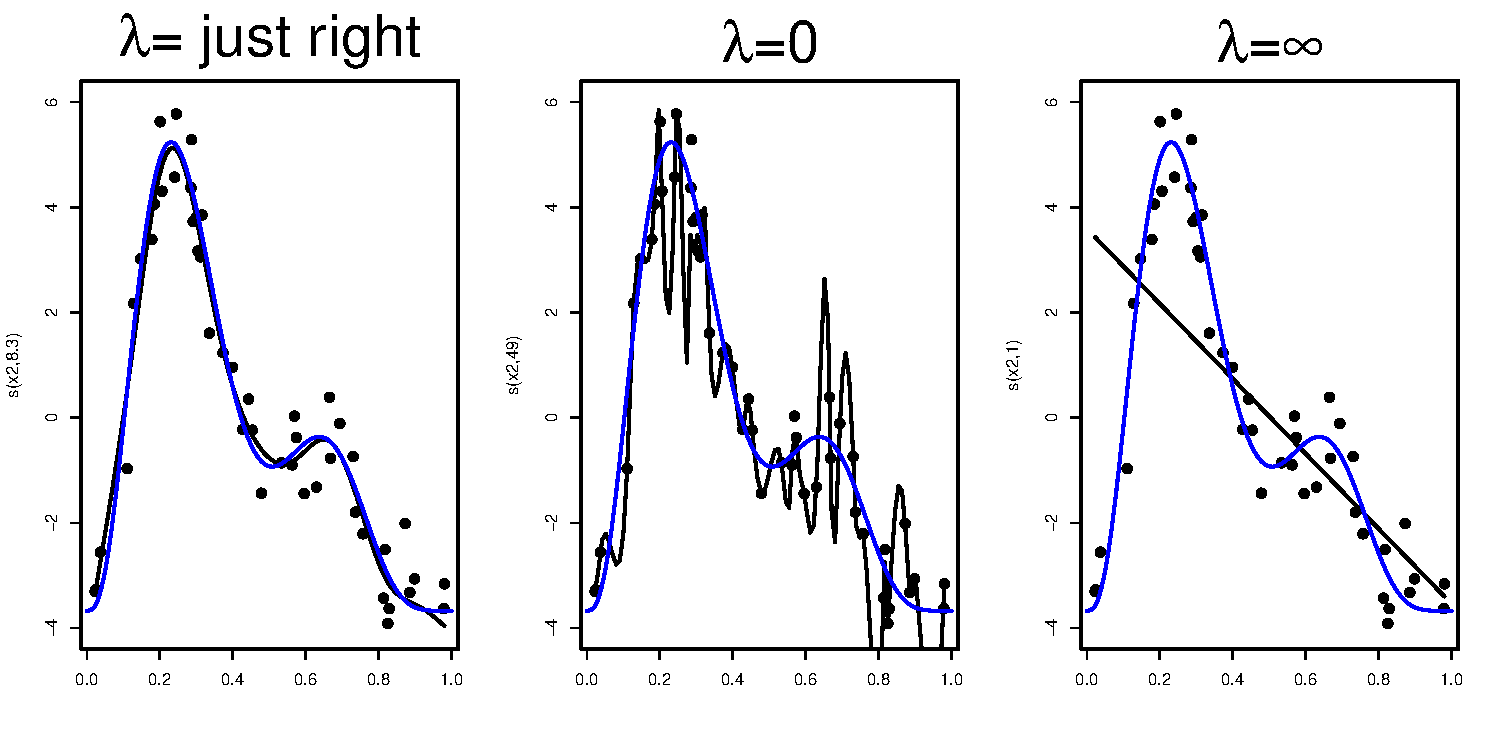
\includegraphics[width=\textwidth]{figures/penalty.pdf}
    \end{center}
  \end{figure}
\end{frame}



%
%\begin{frame}{Smoothing matrix $\bm{S}$}
%\begin{figure}[h]
%  \begin{center}
%    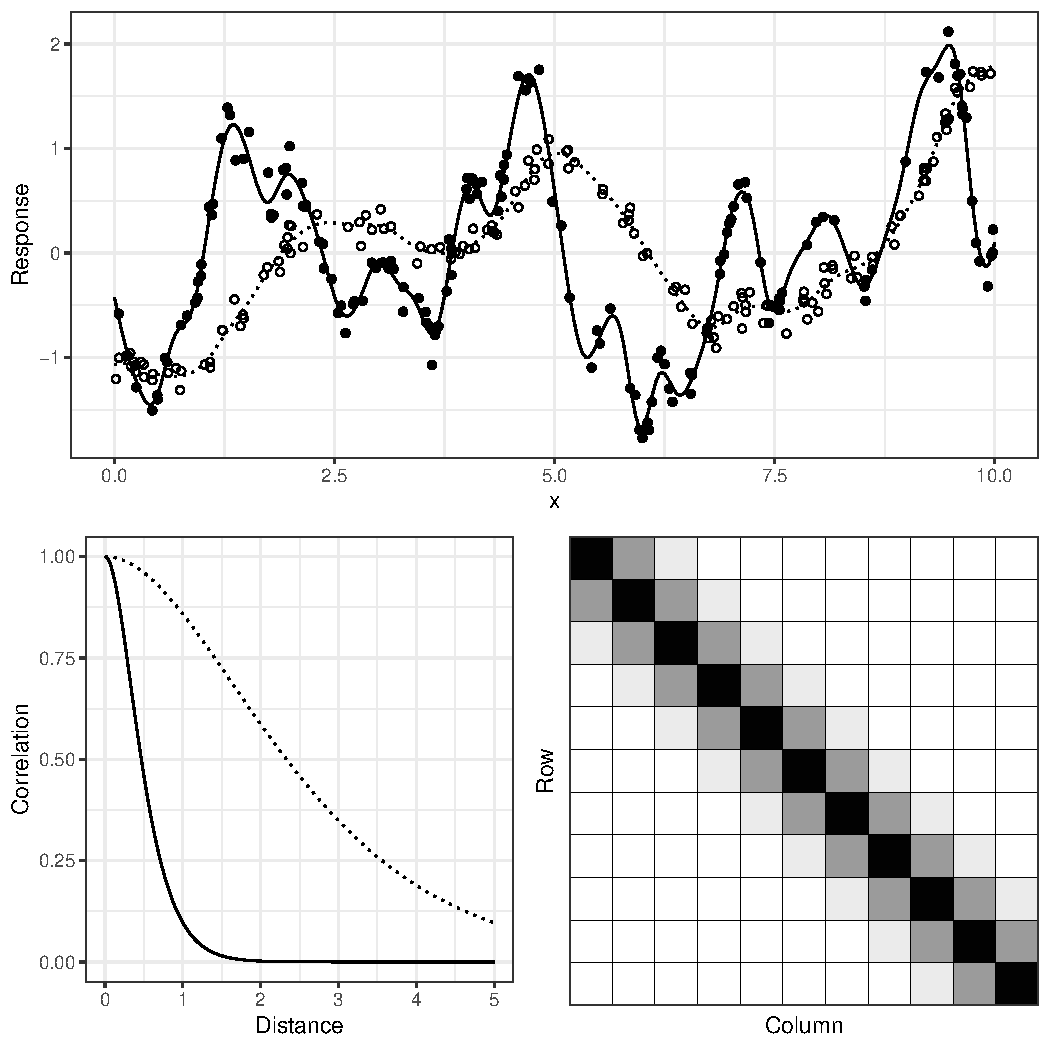
\includegraphics[width=0.7\textwidth, trim={0 9cm 0 0}, clip]{figures/smooth_corr.pdf}
%  \end{center}
%\end{figure}
%  \begin{figure}[h]
%  \begin{center}
%    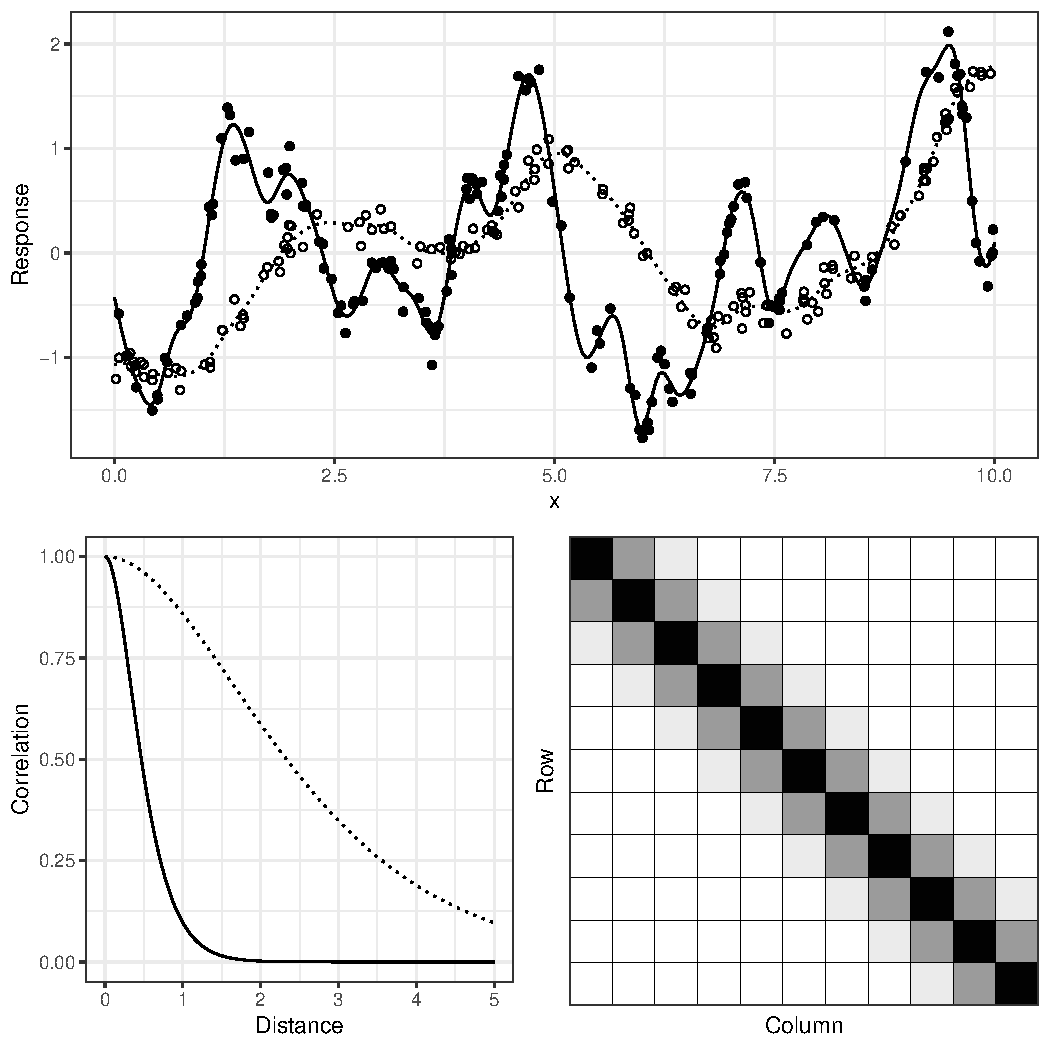
\includegraphics[height=0.4\textheight, trim={9cm 0 0 9cm}, clip]{figures/smooth_corr.pdf}
%  \end{center}
%\end{figure}
%\end{frame}
%
% Richard's section
\section{SPDE approach}

\begin{frame}{Lindgren et al, 2011} 
  \begin{figure}[h]
    \begin{center}
      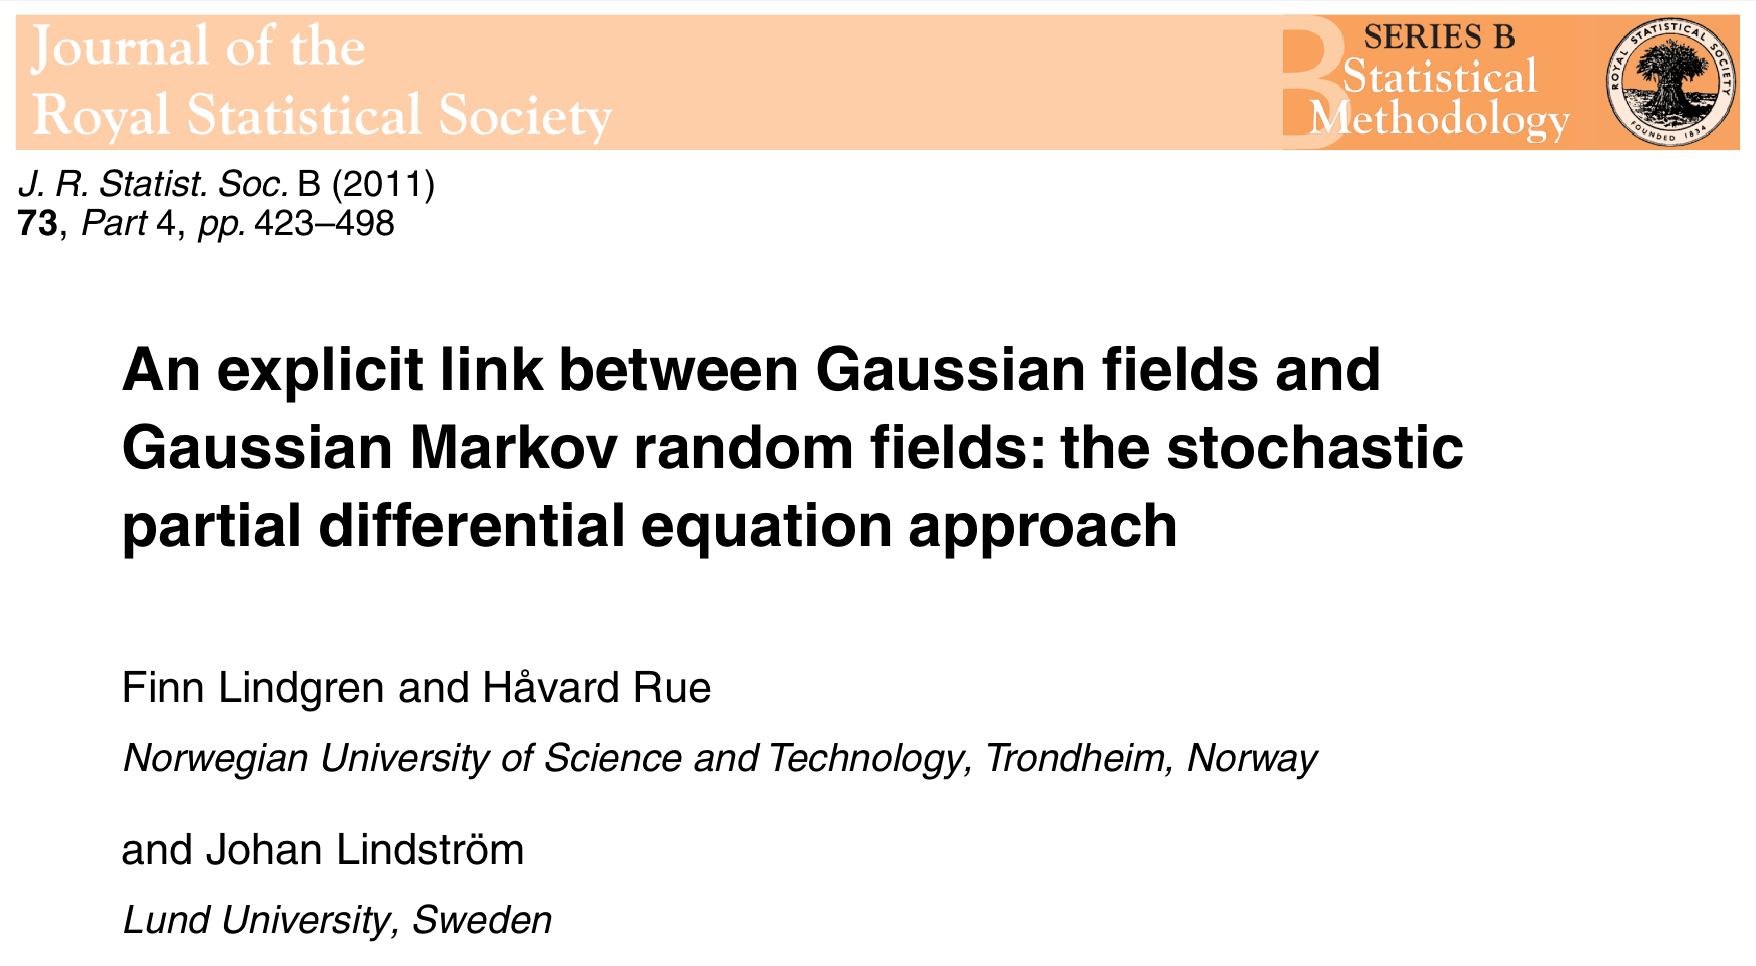
\includegraphics[width=0.9\textwidth]{figures/lindgren.png}
    \end{center}
  \end{figure}
\end{frame}

%
%\begin{frame}{Basic Idea} 
%
%SPDE sets the variance for the rate of change of the underlying curve. 
%
%  \begin{figure}[h]
%    \begin{center}
%      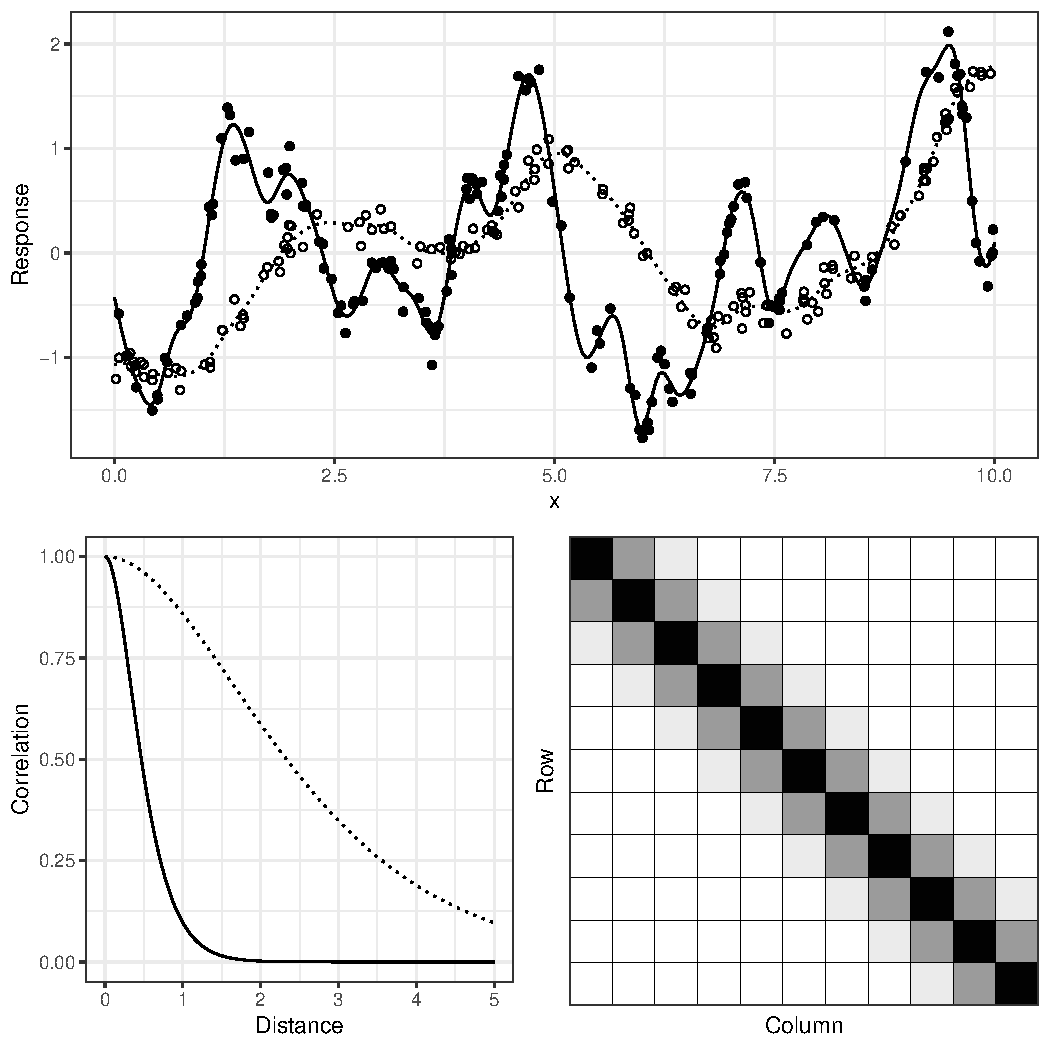
\includegraphics[width=0.7\textwidth, trim={0 9cm 0 0}, clip]{figures/smooth_corr.pdf}
%    \end{center}
%  \end{figure}
%{\Large
%Higher variance in gradient $=$ more wiggly. 
%}
%\end{frame}

\begin{frame}{Two Selling points of SPDE approach} 

1. A certain kind of SPDE produces curves that have Mat\'ern correlation functions, a popular choice of correlation function. 

  \begin{figure}[h]
  \begin{figure}[h]
    \begin{center}
      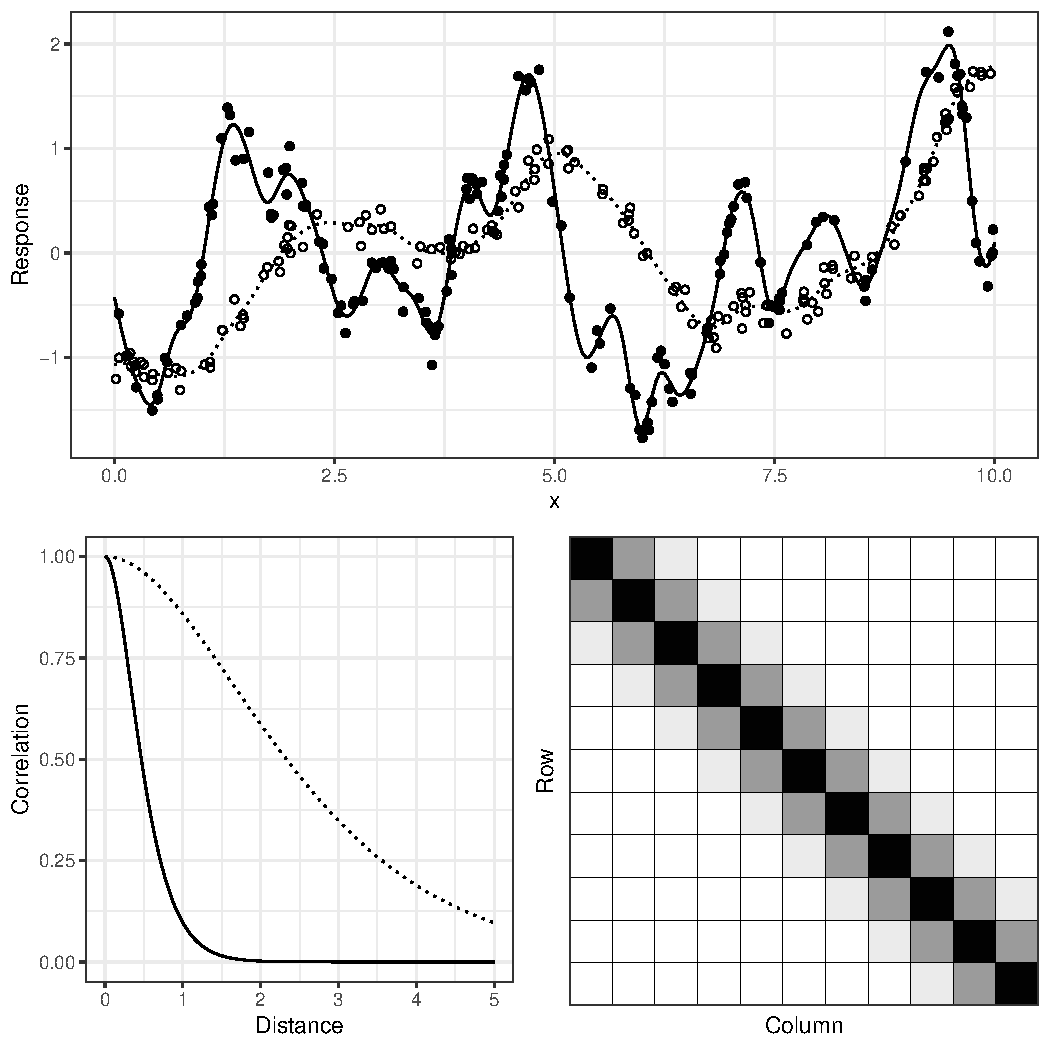
\includegraphics[height=0.4\textheight, trim={0 9cm 0 0}, clip]{figures/smooth_corr.pdf}
    \end{center}
  \end{figure}
    \begin{figure}[h]
    \begin{center}
      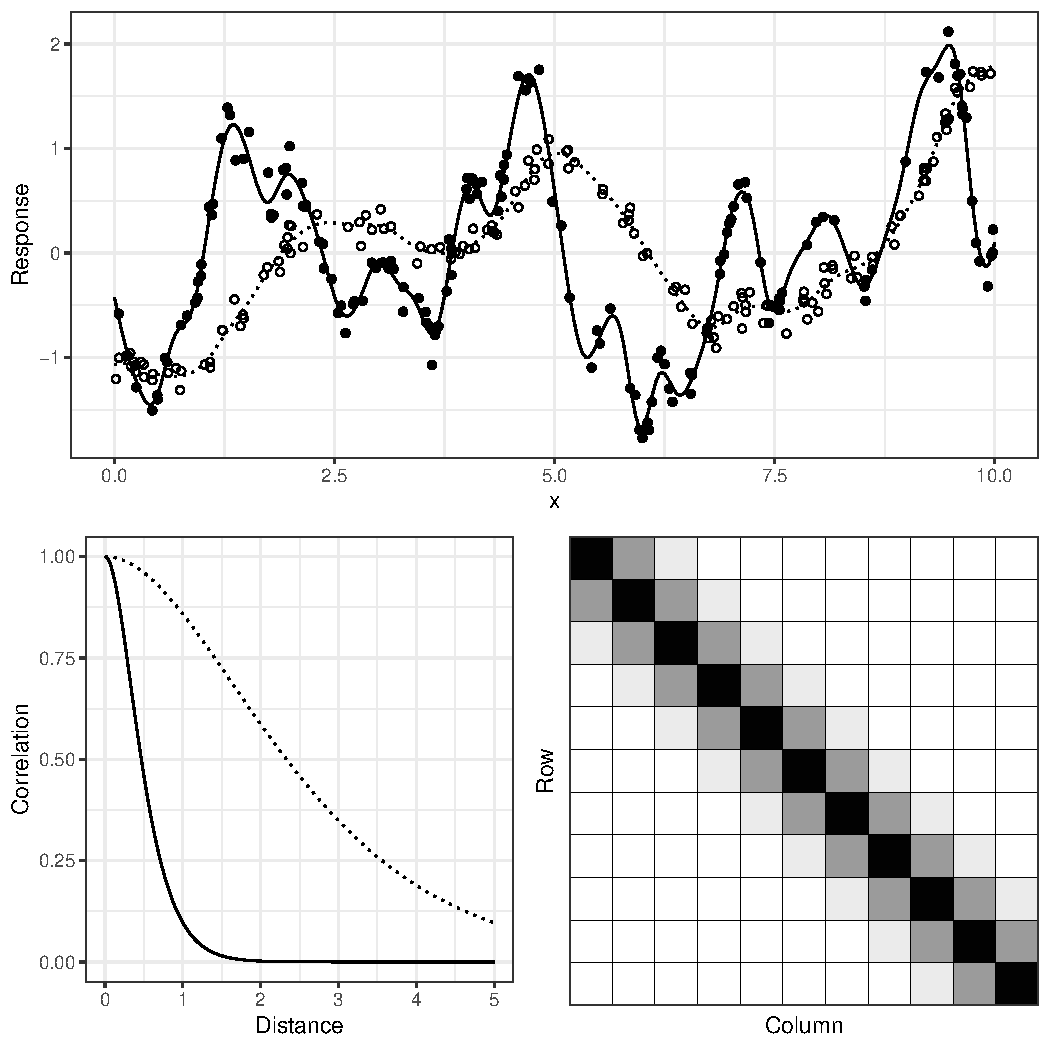
\includegraphics[height=0.35\textheight, trim={0 0 9cm 9cm}, clip]{figures/smooth_corr.pdf}
    \end{center}
  \end{figure}
  \end{figure}

\end{frame}

\begin{frame}{Two Selling points of SPDE approach} 

2. The precision matrix $Q$ can be computed very efficiently, a bottleneck in many other correlation approaches.

  \begin{figure}[h]
    \begin{center}
      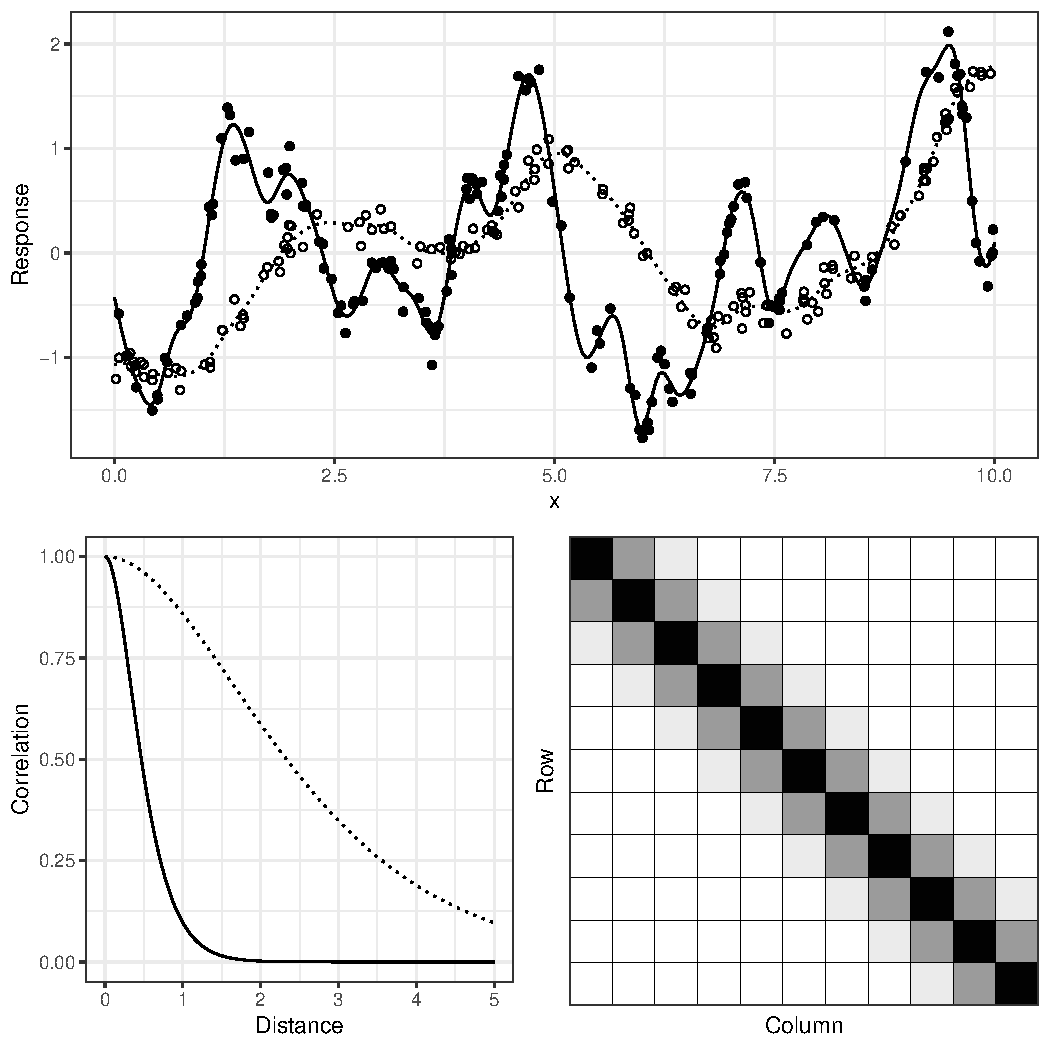
\includegraphics[height=0.7\textheight]{figures/smooth_corr.pdf}
    \end{center}
  \end{figure}

\end{frame}

\begin{frame}{SPDE method comes in 2 bits\ldots}
  \begin{columns}[T]
    \begin{column}{0.40\textwidth}
      \textbf{finite elements}
      \begin{itemize}
        \item join together to make up the overall curve
        \item go in the predictor matrix, $\textbf{A}$
      \end{itemize}
    \end{column}
    \begin{column}{0.58\textwidth}
      \textbf{precision}
      \begin{itemize}
        \item controls how the curve behaves
        \item precision matrix $\textbf{Q}$ (structure)
        \item correlation parameter $\kappa$ (how wiggly)
        \item variance parameter $\tau$ 
      \end{itemize}
    \end{column}
  \end{columns}
\end{frame}

%\begin{frame}{Finite Element}
%  \begin{figure}[h]
%    \begin{center}
%      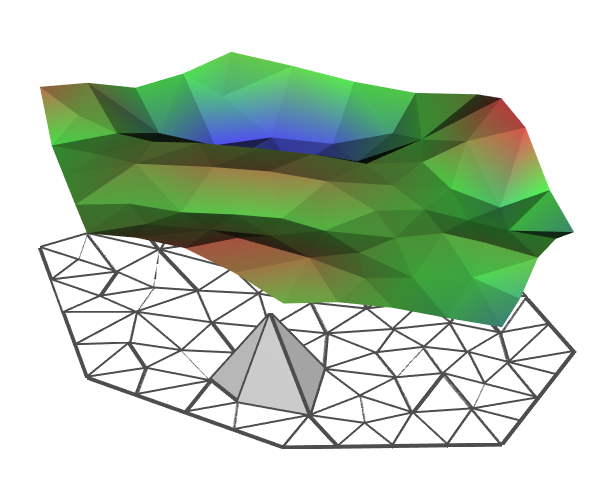
\includegraphics[width=\textwidth]{figures/fcn2.png}
%    \end{center}
%  \end{figure}
%\end{frame}
%
%\begin{frame}{Correlation parameter}
%  \begin{figure}[h]
%    \begin{center}
%      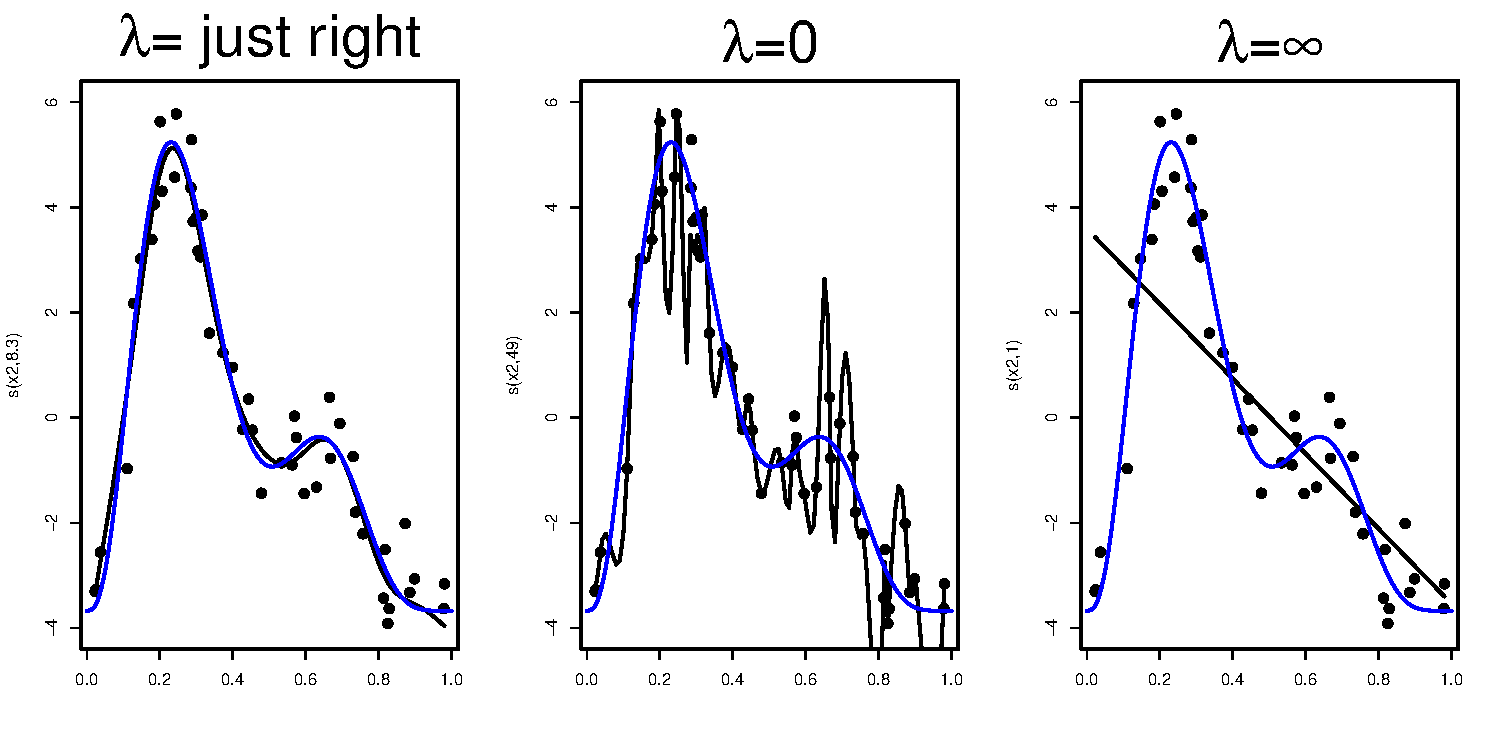
\includegraphics[width=\textwidth, trim={0 0 0 1.2cm}, clip]{figures/penalty.pdf}
%    \end{center}
%  \end{figure}
%\end{frame}
%
%\begin{frame}{Precision matrix $\bm{Q}$}
%  \begin{figure}[h]
%    \begin{center}
%      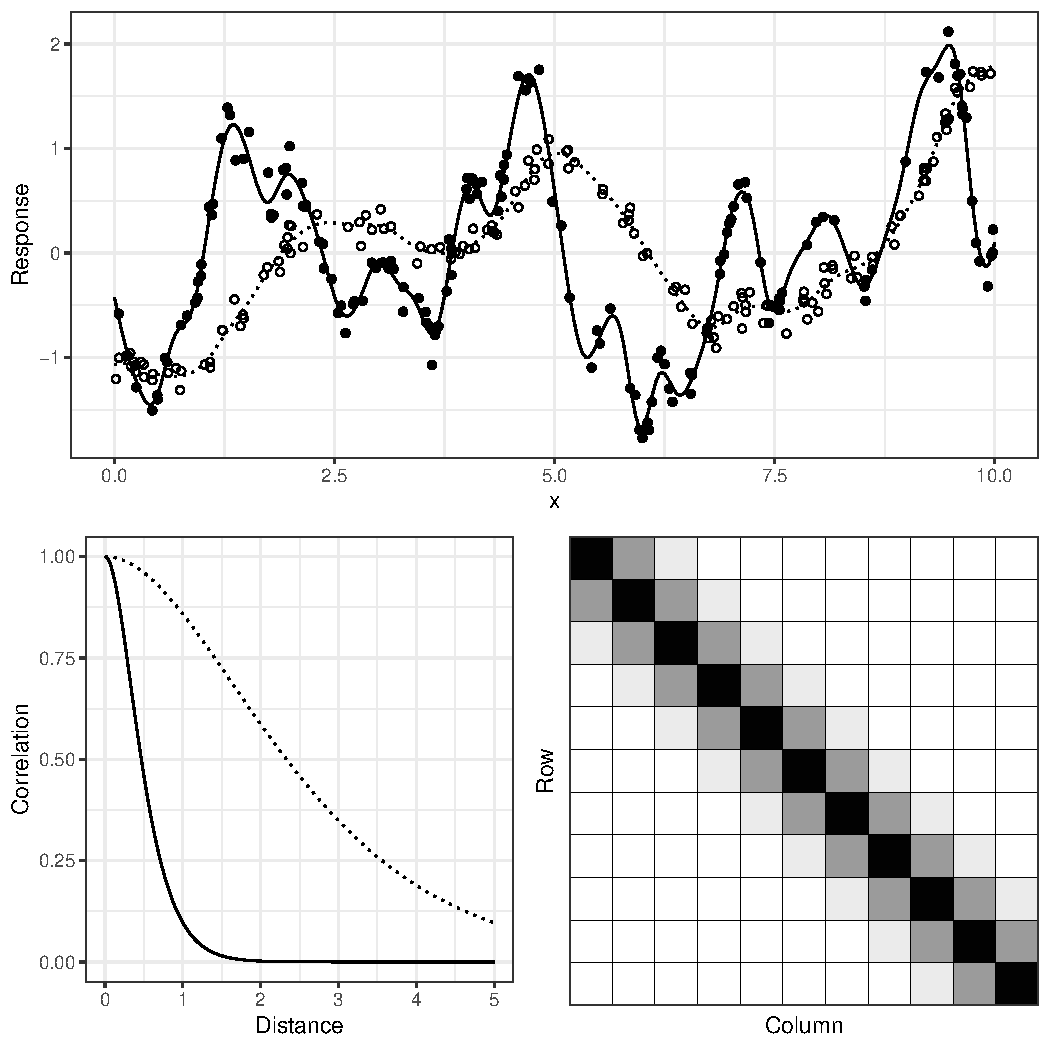
\includegraphics[width=0.7\textwidth, trim={0 9cm 0 0}, clip]{figures/smooth_corr.pdf}
%    \end{center}
%  \end{figure}
%    \begin{figure}[h]
%    \begin{center}
%      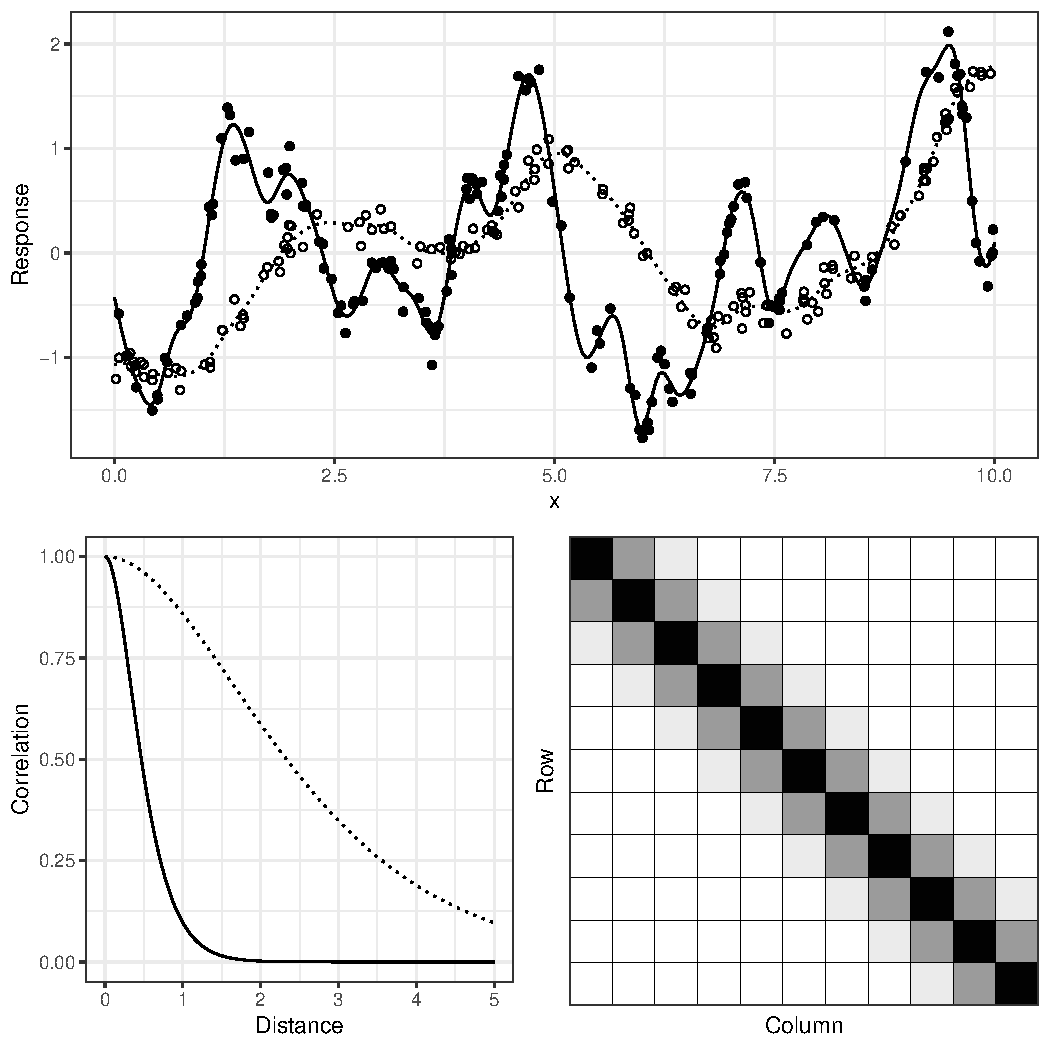
\includegraphics[height=0.4\textheight, trim={9cm 0 0 9cm}, clip]{figures/smooth_corr.pdf}
%    \end{center}
%  \end{figure}
%\end{frame}

\begin{frame}

{\Huge Wait a minute...}
\end{frame}

\begin{frame}{SPDE method comes in 2 bits\ldots}
  \begin{columns}[T]
    \begin{column}{0.40\textwidth}
      {\color{gray} \textbf{\sout{finite elements}}}\\
      \textbf{basis functions}
      \begin{itemize}
        \item join together to make up the overall curve
        \item go in the {\color{gray} predictor} design matrix, $\textbf{A} = \bm{X}$ 
      \end{itemize}
    \end{column}
    \begin{column}{0.58\textwidth}
      {\color{gray} \sout{\textbf{precision}}}\\
      \textbf{penalty}
      \begin{itemize}
        \item controls how the curve behaves
        \item precision matrix $\textbf{Q} = \bm{S}$ (structure)
        \item {\color{gray} correlation parameter $\kappa$ (how wiggly)
        \item variance parameter $\tau$ } 
        \item $\kappa, \tau \leadsto \lambda$ 
      \end{itemize}
    \end{column}
  \end{columns}
\end{frame}

\begin{frame}{SPDE is a basis-penalty smoother}

{\Large
The SPDE has a corresponding smoothness penalty.

Pick same basis, then 
$$ \bm{A} = \bm{X}  $$

Use SPDE and corresponding penalty, then 
$$ \bm{Q} = \bm{S} $$
}

\small{See our paper for more mathematical details.}
\end{frame}

\begin{frame}{The SPDE method is a basis-penalty smoother}
\begin{figure}
\resizebox{\textwidth}{!}{
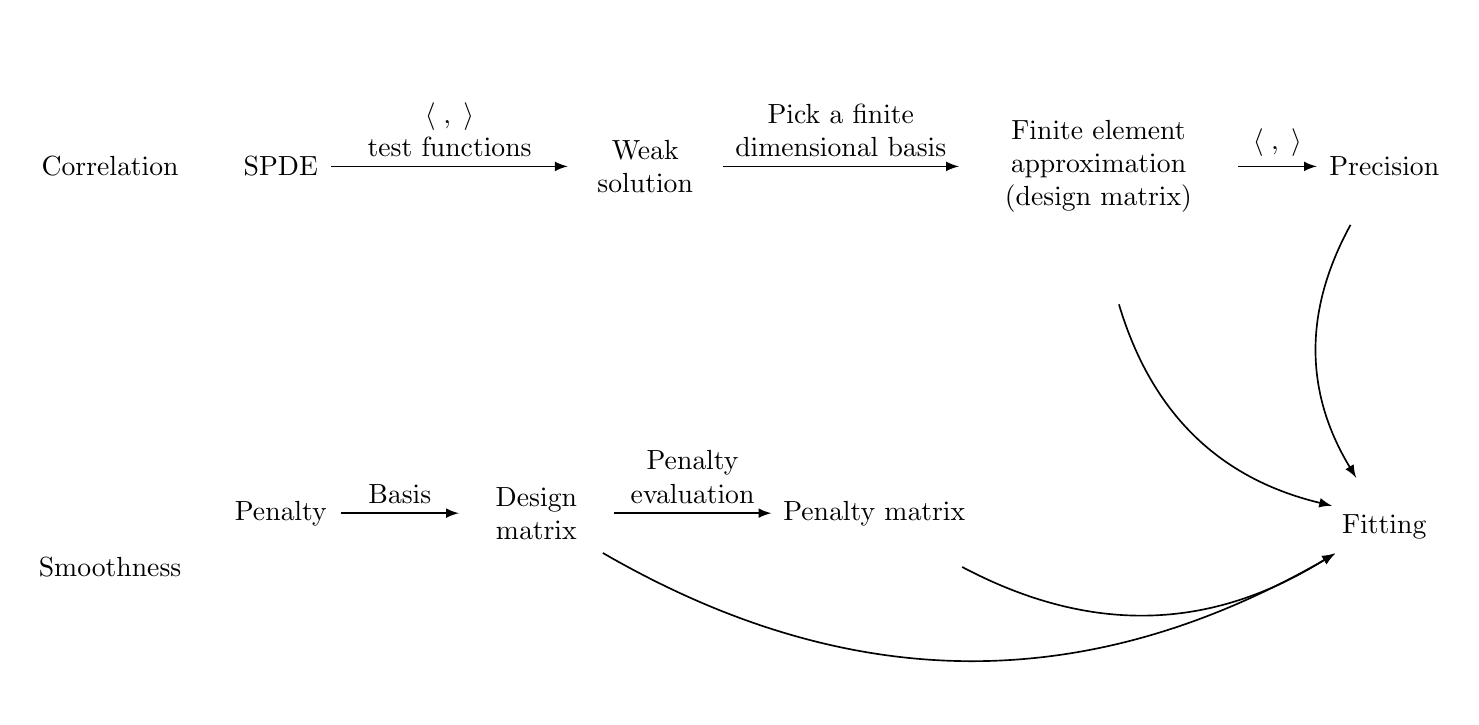
\begin{tikzpicture}[-latex, auto, node distance=3cm and 2cm, semithick,
                    state/.style ={circle, minimum width =0.5 cm}, every text node part/.style={align=center}]

% SPDE nodes
\node[state] (corr) {Correlation};
\node[state] (spde) [right=.5cm of corr] {SPDE};
\node[state] (weak) [right =3cm of spde, text width=1.5cm] {Weak solution};
\node[state] (fem) [right =3cm of weak, text width=3cm] {Finite element approximation (design matrix)};
\node[state] (prec) [right =1cm of fem] {Precision};
\node[state] (model) [below =of prec] {Fitting};

% GAM nodes
\node[state] (smoothness) [below= of corr] {Smoothness};
\node[state] (pen) [below=of spde] {Penalty};
\node[state] (pdesol) [right=1.5cm of pen, text width=1.5cm] {Design matrix};
\node[state] (penalty) [right=of pdesol] {Penalty matrix};

% spde edges
\path (spde) edge [right] node[above] {$\langle \;,\; \rangle$ \\ test functions} (weak);
\path (weak) edge [right] node[above] {Pick a finite \\ dimensional basis} (fem);
\path (fem) edge [right] node[above] {$\langle \;,\; \rangle$} (prec);
\path (prec) edge [bend right] node[above] {} (model);
\path (fem) edge [bend right] node[above] {} (model);

% GAM
\path (pen) edge [right] node[above] {Basis} (pdesol);
\path (pdesol) edge [right] node[above] {Penalty \\ evaluation} (penalty);
\path (penalty) edge [bend right] node[above] {} (model);
\path (pdesol) edge [bend right] node[above] {} (model);

\end{tikzpicture}
}

\label{fig:flow}
\end{figure}
\end{frame}

\section{Practical implications}
\begin{frame}{What about R-INLA and mgcv?}
  \begin{itemize}
   \item Both are ways to fit this same model.   
    \item Both \texttt{R-INLA} and \texttt{mgcv} do approximations:
    \begin{itemize}
    		\item \texttt{R-INLA} does a Laplace approximation to get around MCMC.
 	    \item \texttt{mgcv} does REML using Laplace approximation too.
	\end{itemize}
    	\item \texttt{mgcv} does empirical Bayes, so uses point estimates for hyperparameters (smoothing parameters, variance components). 
    \item (\texttt{R-INLA} can do this too!)
  \end{itemize}
\end{frame}

\begin{frame}{What can we do with this?}
  \begin{itemize}
	\item Writing SPDE models as basis-penalty smoothers means we can use them elsewhere
 	\item Anywhere structured random effects can be used!
	\item \texttt{mgcv}, \texttt{TMB}, Stan, etc
	\item We can combine them with other approaches!
  \end{itemize}
\end{frame}

\begin{frame}{\textit{mgcv} code}
Setup using \texttt{R-INLA}, fit with \texttt{mgcv}
		\begin{figure}
		\begin{center}
			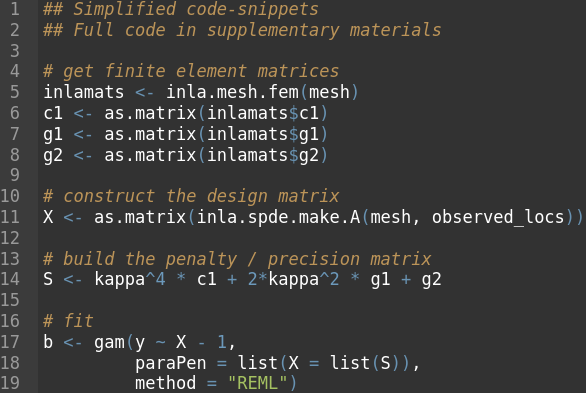
\includegraphics[scale = 0.5]{figures/mgcvcode.png}
		\end{center}
	\end{figure}
\end{frame}

\begin{frame}{1D comparison}
	\begin{figure}
		\begin{center}
			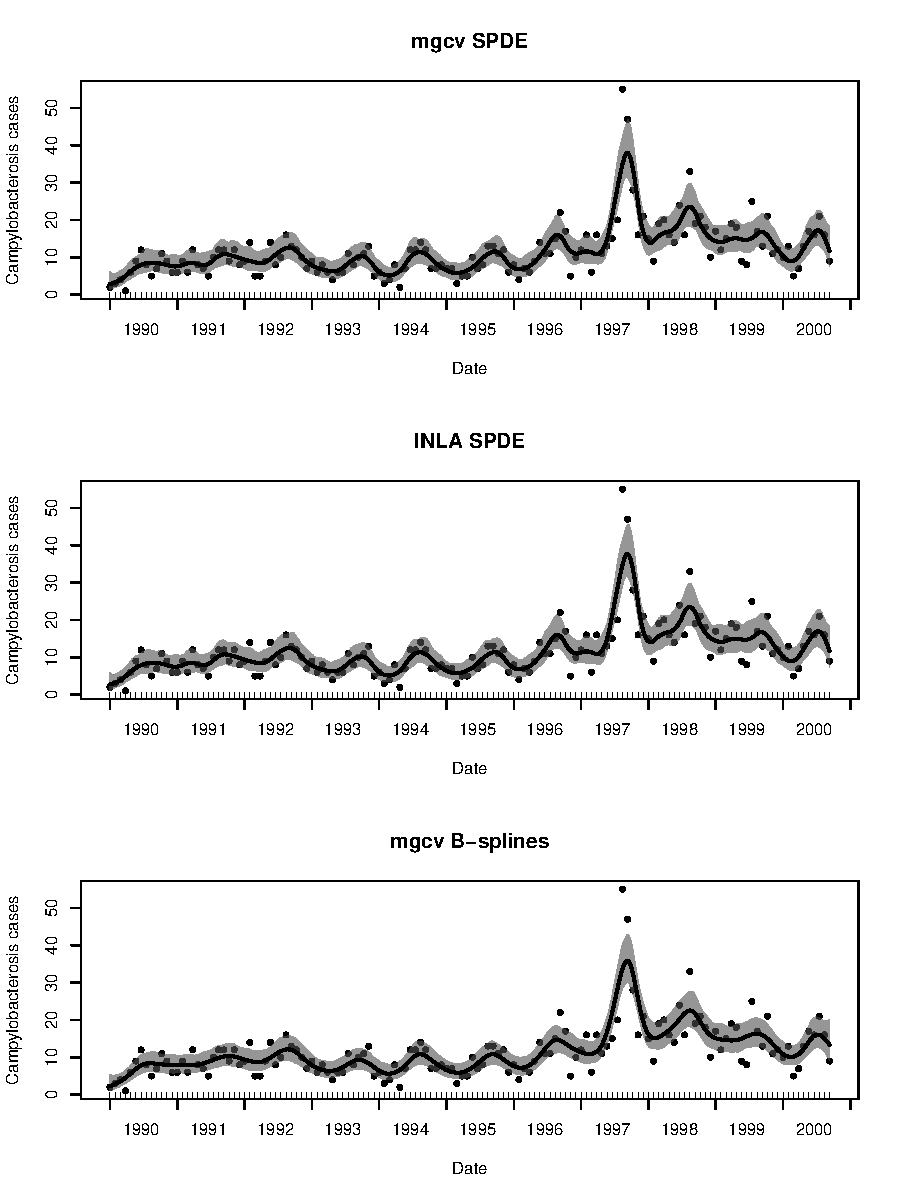
\includegraphics[height = 0.95\textheight]{figures/campy.pdf}		
		\end{center}
	\end{figure}
\end{frame}


\begin{frame}{Spatial smoothing comparison}
	\begin{figure}
		\begin{center}
			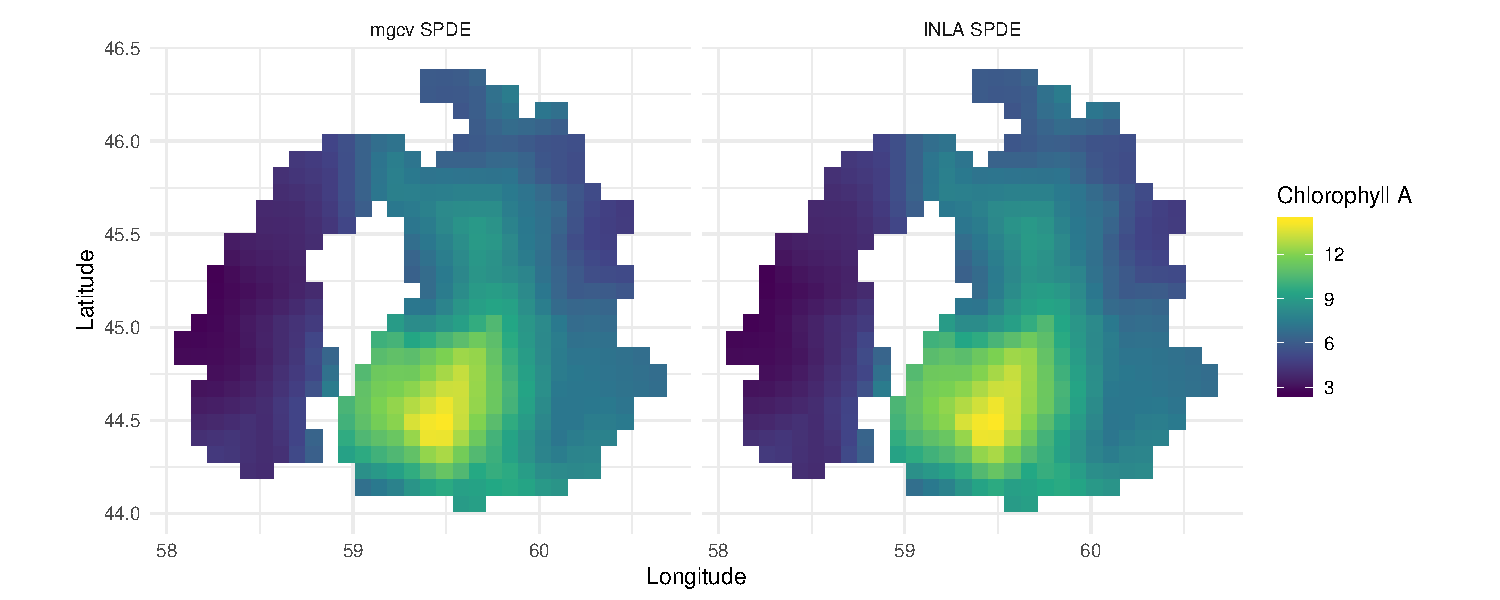
\includegraphics[scale = 0.45]{figures/aral.pdf}		
		\end{center}
	\end{figure}
\end{frame}


%\begin{frame}{Case Study}
%
%Point counts of a Hawaiian honeycreeper (Akepa)
%
%\begin{figure}[h]
%    \begin{center}
%      \includegraphics[height=0.7\textheight]{figures/akepa_transects.png}
%    \end{center}
%  \end{figure}
%
%\end{frame}
%
%\begin{frame}{Basis functions} 
%
%\begin{figure}[h]
%    \begin{center}
%      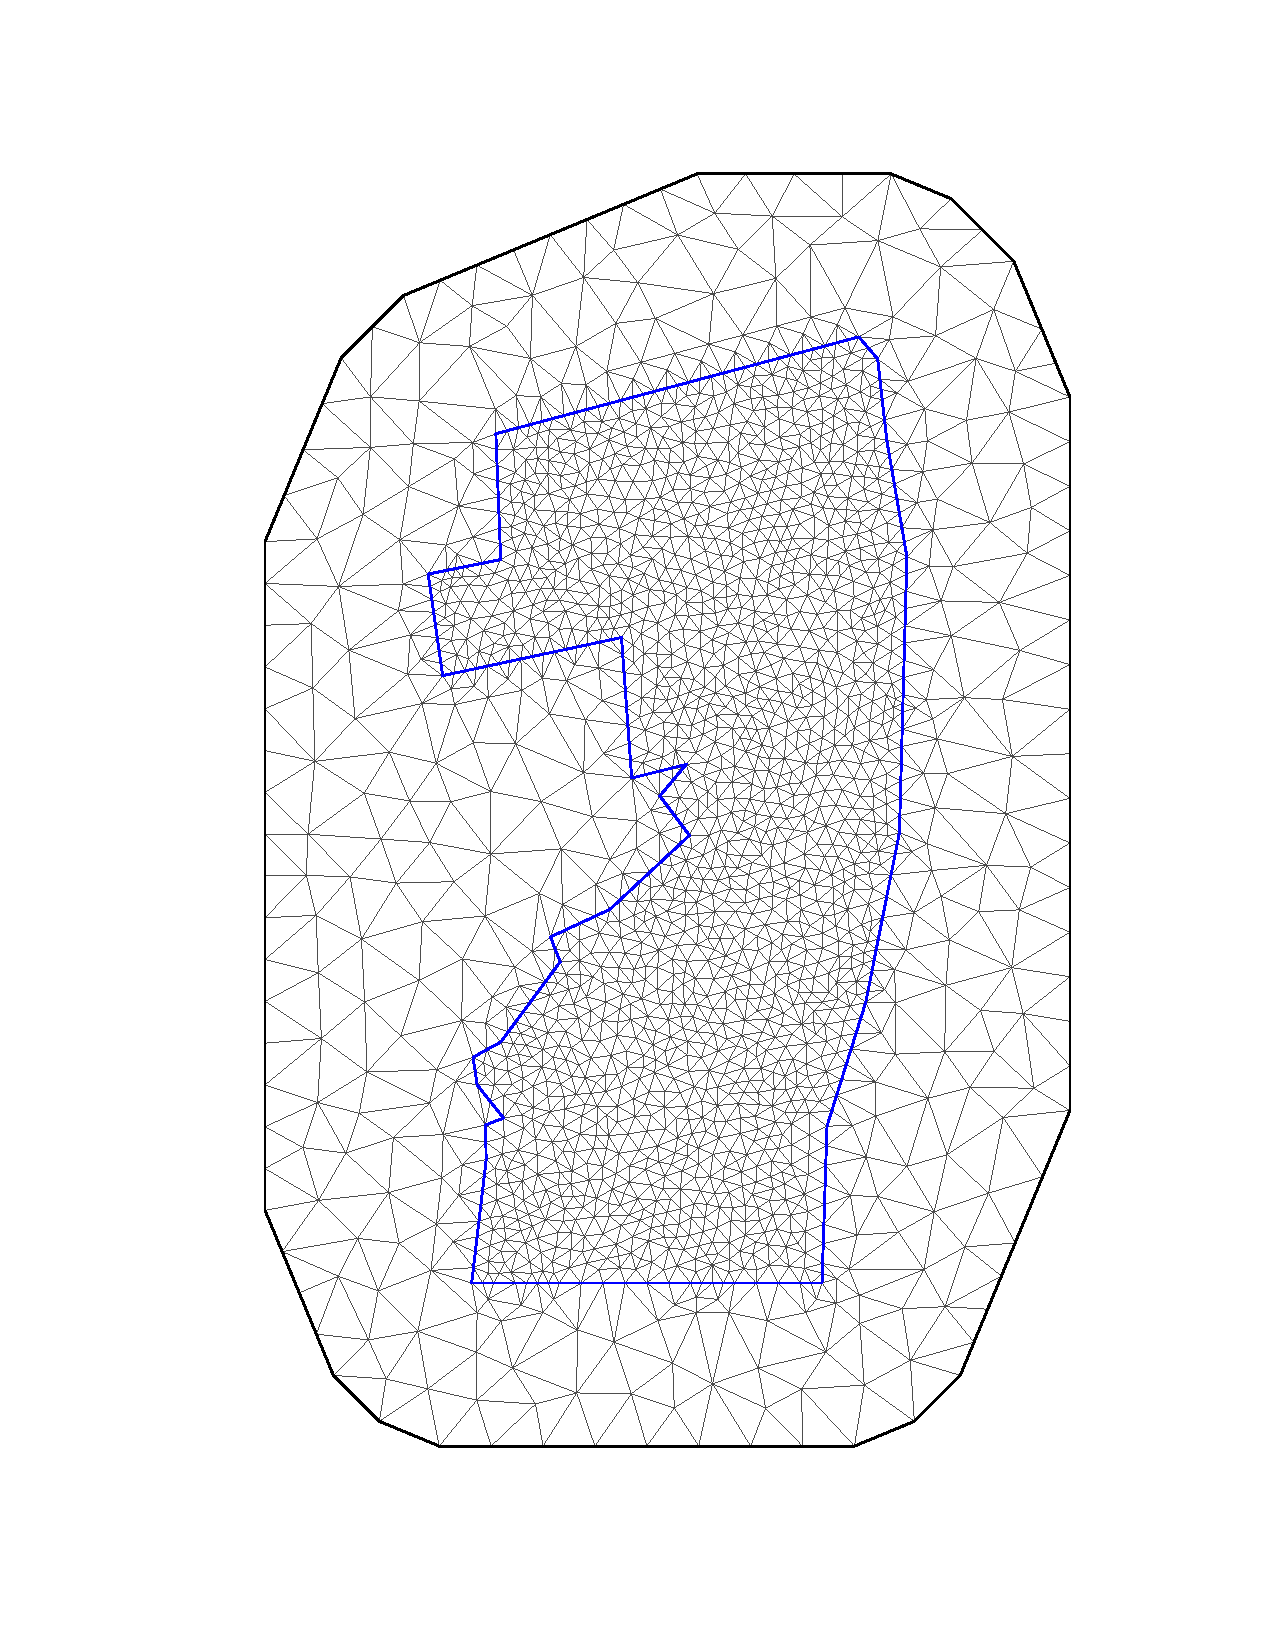
\includegraphics[height=0.9\textheight]{figures/mesh.pdf}
%    \end{center}
%  \end{figure}
%
%\end{frame}


%\begin{frame}{Case Study - TPRS vs. SPDE}
%\begin{figure}[h]
%    \begin{center}
%      \includegraphics[height=0.95\textheight]{figures/akepa_comparison.png}
%    \end{center}
%  \end{figure}
%\end{frame}

\section{Take-home}

\begin{frame}{A modelling framework emerges}

Use basis-penalty or basis-precision as a common currency.

\begin{enumerate}
 \item \textbf{Choose a covariance model}: explicitly (as in kriging, etc), via smoothness penalty (e.g., splines), or with an SPDE;
 \item \textbf{Approximate the precision matrix \(Q\)}: reduce dimension or induce sparsity in \(Q\);
 \item \textbf{Draw approximate inference using a software implementation}: e.g., with \texttt{mgcv}, MCMC (e.g., Stan; \texttt{JAGS}), \texttt{R-INLA}, \texttt{lme4}  or \texttt{TMB}.
\end{enumerate}

\end{frame}



\section{More info?}

\begin{frame}{DOI \texttt{10.1007/s13253-019-00377-z}}
  \begin{figure}[htbp]
    \begin{center}
      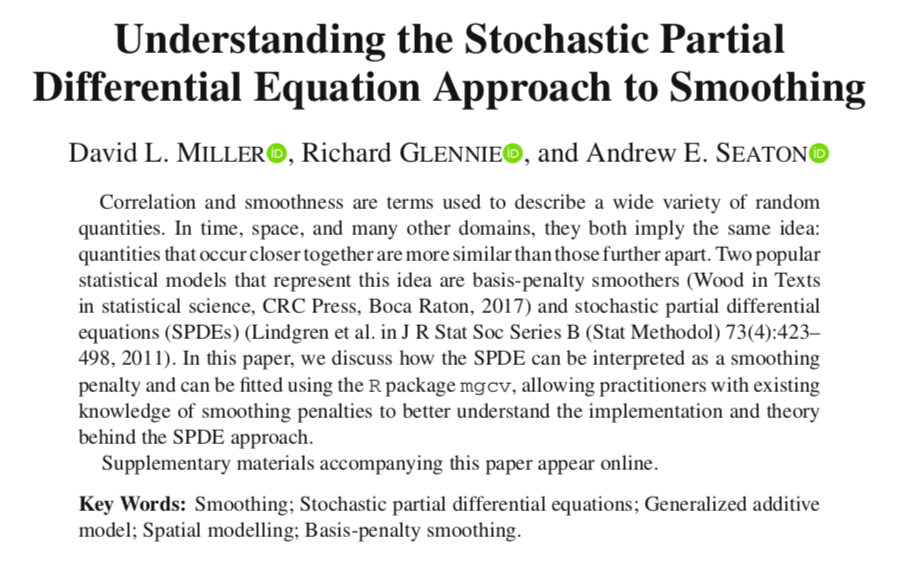
\includegraphics[width=0.9\textwidth]{figures/paper.png}
    \end{center}
  \end{figure}
  \begin{center}
  Slides: \url{https://github.com/dill/SPDE-talk-IBS}
  \end{center}
  
\end{frame}

%\begin{frame}{Bonus Scooby}
%  \begin{figure}[htbp]
%    \begin{center}
%      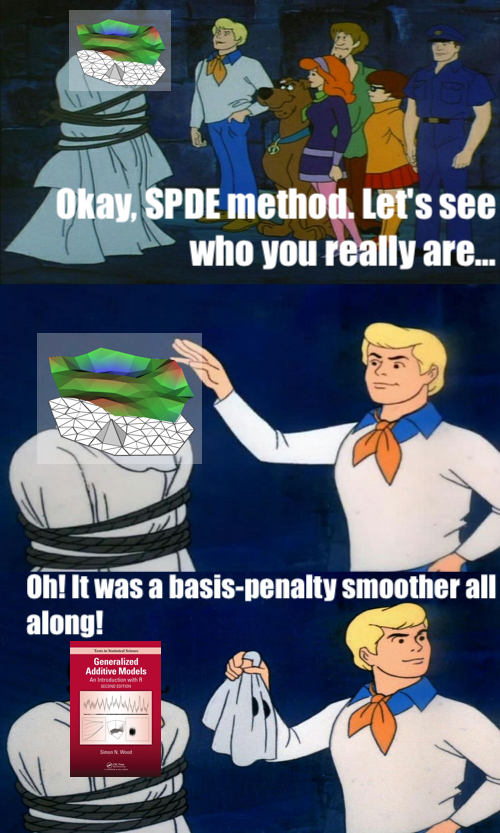
\includegraphics[height=0.4\textheight, trim={0 19.5cm 0 0}, clip]{figures/scooby.png}
%    \end{center}
%  \end{figure}
%    \begin{figure}[htbp]
%    \begin{center}
%      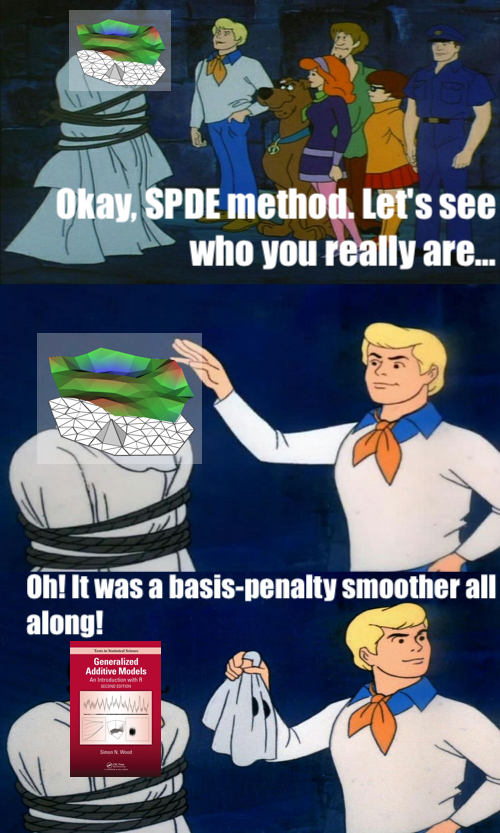
\includegraphics[height=0.4\textheight, trim={0 0 0 20.25cm}, clip]{figures/scooby.png}
%    \end{center}
%  \end{figure}
%\end{frame}
%

\end{document}
